
%% bare_conf.tex
%% V1.3
%% 2007/01/11
%% by Michael Shell
%% See:
%% http://www.michaelshell.org/
%% for current contact information.
%%
%% This is a skeleton file demonstrating the use of IEEEtran.cls
%% (requires IEEEtran.cls version 1.7 or later) with an IEEE conference paper.
%%
%% Support sites:
%% http://www.michaelshell.org/tex/ieeetran/
%% http://www.ctan.org/tex-archive/macros/latex/contrib/IEEEtran/
%% and
%% http://www.ieee.org/

%%*************************************************************************
%% Legal Notice:
%% This code is offered as-is without any warranty either expressed or
%% implied; without even the implied warranty of MERCHANTABILITY or
%% FITNESS FOR A PARTICULAR PURPOSE! 
%% User assumes all risk.
%% In no event shall IEEE or any contributor to this code be liable for
%% any damages or losses, including, but not limited to, incidental,
%% consequential, or any other damages, resulting from the use or misuse
%% of any information contained here.
%%
%% All comments are the opinions of their respective authors and are not
%% necessarily endorsed by the IEEE.
%%
%% This work is distributed under the LaTeX Project Public License (LPPL)
%% ( http://www.latex-project.org/ ) version 1.3, and may be freely used,
%% distributed and modified. A copy of the LPPL, version 1.3, is included
%% in the base LaTeX documentation of all distributions of LaTeX released
%% 2003/12/01 or later.
%% Retain all contribution notices and credits.
%% ** Modified files should be clearly indicated as such, including  **
%% ** renaming them and changing author support contact information. **
%%
%% File list of work: IEEEtran.cls, IEEEtran_HOWTO.pdf, bare_adv.tex,
%%                    bare_conf.tex, bare_jrnl.tex, bare_jrnl_compsoc.tex
%%*************************************************************************

% *** Authors should verify (and, if needed, correct) their LaTeX system  ***
% *** with the testflow diagnostic prior to trusting their LaTeX platform ***
% *** with production work. IEEE's font choices can trigger bugs that do  ***
% *** not appear when using other class files.                            ***
% The testflow support page is at:
% http://www.michaelshell.org/tex/testflow/



% Note that the a4paper option is mainly intended so that authors in
% countries using A4 can easily print to A4 and see how their papers will
% look in print - the typesetting of the document will not typically be
% affected with changes in paper size (but the bottom and side margins will).
% Use the testflow package mentioned above to verify correct handling of
% both paper sizes by the user's LaTeX system.
%
% Also note that the "draftcls" or "draftclsnofoot", not "draft", option
% should be used if it is desired that the figures are to be displayed in
% draft mode.
%
\documentclass[conference]{IEEEtran}
% Add the compsoc option for Computer Society conferences.

\usepackage[utf8]{inputenc}
\usepackage[english]{babel}
\usepackage[T1]{fontenc}

% CITATION PACKAGES
\usepackage{cite}

% GRAPHICS RELATED PACKAGES
\ifCLASSINFOpdf
  \usepackage[pdftex]{graphicx}
  % declare the path(s) where your graphic files are
  \graphicspath{{aux/}}
  \DeclareGraphicsExtensions{.pdf,.jpeg,.png}
\else
  \usepackage[dvips]{graphicx}
  \graphicspath{{aux/}}
  \DeclareGraphicsExtensions{.eps}
\fi

% MATH PACKAGES
\usepackage[cmex10]{amsmath}
\interdisplaylinepenalty=2500

% SPECIALIZED LIST PACKAGES
\usepackage{algorithmic}

% ALIGNMENT PACKAGES
\usepackage{array}
\usepackage{mdwmath}
\usepackage{mdwtab}
\usepackage{eqparbox}

% SUBFIGURE PACKAGES
\usepackage[caption=false,font=footnotesize]{subfig}
\usepackage{multirow,tabularx}

% FLOAT PACKAGES
\usepackage{fixltx2e}
\usepackage{stfloats}
\usepackage{float}

% PDF, URL AND HYPERLINK PACKAGES
\usepackage{url}

% fix search and cut-and-paste in Acrobat
\usepackage{cmap}
\usepackage{ifthen}
% place figures here definitely
\floatplacement{figure}{H}
%\setcounter{secnumdepth}{0}

% Multi-column tables
\usepackage{multirow,tabularx}

% hyperlinks:
\ifthenelse{\isundefined{\hypersetup}}{
  \usepackage[colorlinks=true,linkcolor=blue,urlcolor=blue]{hyperref}
  \urlstyle{same} % normal text font (alternatives: tt, rm, sf)
}{}
\hypersetup{
  pdftitle={Visual Odometry for Autonomous Underwater Vehicles},
}

% correct bad hyphenation here
\hyphenation{op-tical net-works semi-conduc-tor}

\begin{document}

% paper title
\title{Visual Odometry for Autonomous Underwater Vehicles}

% author names and affiliations
\author{\IEEEauthorblockN{Stephan Wirth}
\IEEEauthorblockA{System, Robotics and Vision Group\\
Universitat de les Illes Balears\\
Palma de Mallorca, Spain\\
Email: stephan.wirth@uib.es}
\and
\IEEEauthorblockN{Pep Lluis Negre Carrasco}
\IEEEauthorblockA{System, Robotics and Vision Group\\
Universitat de les Illes Balears\\
Palma de Mallorca, Spain\\
Email: pl.negre@uib.cat} 
\and
\IEEEauthorblockN{Gabriel Oliver Codina}
\IEEEauthorblockA{System, Robotics and Vision Group\\
Universitat de les Illes Balears\\
Palma de Mallorca, Spain\\
Email: goliver@uib.es}}

% make the title area
\maketitle


\begin{abstract}
Vision based motion estimation algorithms are widely used in ground-based and aerial robotics. Combined with inertial measurement units, they have proven to be a precise and low-cost sensor for velocity and pose estimation. In this paper we show that stereo vision based odometry can be used by autonomous underwater vehicles that navigate close to the seabed for velocity and incremental pose estimation in small areas. We present the integration of two different stereo visual odometry algorithms into an AUV and experiments carried out in laboratory and harbour conditions comparing vision based pose estimates with ground truth.
\end{abstract}


\section{Introduction 
  \label{introduction}
}

The lastest advances in Autonomous Underwater Vehicles (AUVs) demand accurate estimations of the vehicle's pose and velocity. The tasks to be performed by such robots are increasingly complex and, in most cases it is needed to precisely positioning the underwater vehicle to a certain location in order to execute the desired task. Navigation systems based on wirelessly transmited data, such as Global Positioning System (GPS) or mobile network positioning, can not be used in uderwater enviroments. Therefore the AUV must estimate its position using self-contained sensors. One of the most popular positioning sensors for underwater vehicles is the Doppler Velocity Log (DVL) which provides precise velocity and altitude updates for a wide variety of underwater tasks. However, DVL is an expensive device that cannot be integraded in many underwater projects.

Visual odometry is the process of estimating a vehicle 3D pose using only visual images. This technique is becoming popular in AUVs for navigation, station keeping and the provision of a manipulator feedback information. Visual odometry output is often fused with Inertial Measurement Units (IMU) to provide a cheaper alternative to DVLs \cite{Hildebrandt2010}. However, the limitations of underwater vision are widely known, and its performance depends on many factors such as visibility, lighting and distorsion resulting from varying refractive indices.

In this paper we present the integration of two popular stereo visual odometry algorithms into an AUV, the experiments carried out in laboratory and harbour enviroments, as well as the evaluation method to compare the performance of both algorithms.

First, the paper presents related works on visual odometry. Section \ref{visual-odometry-systems} describes the general concepts of visual odometry systems and presents a brief overview of the two analyzed algorithms (fovis and libviso2), followed by the explanation of the evaluation method in Section \ref{evaluation-method} and experiments in different eviroments. Finally, the conclusion ot the study and future prespectives are presented.

\section{Related Work 
  \label{related-work}
}

TODO: Any publications on underwater visual odometry (including AUVs), else UAV or automobile systems


\section{Visual Odometry Systems
  \label{visual-odometry-systems}
}
A visual odometry system consists of one or more cameras, a processing unit, and the required algorithms that process incoming images.
Algorithms for visual odometry - as opposed to full SLAM algorithms - focus on fast frame-to-frame motion estimates without keeping a large history for loop closing. The emphasis lies on accurate measurements at high frequencies. Systems that use just one camera need translational movement for 3D motion estimation and all measurements have to be scaled by an unknown factor to be on a metric scale. Using a calibrated stereo camera overcomes both of the aforementioned problems as 3D coordinates of matched points in a single left/right image pair can be computed by triangulation. We therefore focus our work on visual odometry systems that use stereo cameras.

The two publicly available algorithms we compare are \emph{libviso2} \cite{Geiger2011} and \emph{fovis} \cite{Huang2011}. The former has been successfully used on cars, and the latter has proven to work for micro aerial vehicles.

We created wrappers for both libraries\footnote{See \url{http://www.ros.org/viso2_ros} and \url{http://www.ros.org/fovis_ros} for source code and documentation.} to integrate them into the Robot Operating System ROS \cite{Quigley2009}. This simplifies the integration in different robotic vehicles as well as comparison with other integrated sensors.


Both algorithms have very similar processing pipelines containing feature detection, filtering, matching, and motion estimation. Table \ref{odometry-comparison} summarizes the steps of the algorithms, outlining similarities and differences. To limit the extend of this paper, the interested reader is refered to the original papers for a deeper understanding and more detailed description of the algorithms. In the following we give a brief overview of both algorithms.

\subsection{libviso2
  \label{libviso2}
}

The features used by libviso2 are simple blob and corner detector masks, resulting in a large amount of interest points of four different classes. Non-minima-/non-maxima-suppression is used for initial feature reduction. In this step, two different thresholds for minima/maxima selection are used resulting in two sets of sparse strong features and dense less strong features. This allows for a multi-stage matching coarse to fine using matches of the strong features to limit the search range for the weaker ones. The used descriptor contains only 16 values of sobel filter responses distributed inside an 11x11 pixel window. The similarity measure for two features is the sum of absolute differences of their descriptors. The computation of this measure is sped up using SIMD instructions.

The matching of features follows the following order: current left image to current right image, current right image to previous right image, previous right image to previous left image and previous left image to current right image. If the target feature of the last matching is the same as the source feature of the first matching the match is classified as valid. Apart from the aforementioned search range limitation, possibly wrong matches are discarded using a neighborhood support heuristic.
From the obtained matches a subset is drawn that is distributed over the whole image by dividing the image in a grid of subimages and drawing a fixed maximum number of matches from each cell.

Subsequently, 3D coordinates of the features in the previous image pair are calculated through triangulation. Gauss-Newton minimization of the reprojection error of these 3D points onto the current left and right images leads to the rigid transformation from the previous image's camera pose to the current camera pose. The motion estimation procedure is wrapped in a RANSAC \cite{Fischler1981} scheme.


\subsection{fovis
  \label{fovis}
}

fovis uses the FAST feature detector \cite{Rosten2005FPA,Rosten2006MLF} with an adaptive threshold on three gaussian pyramid levels. The number of features is reduced taking the best features of each cell of a regular grid. The feature descriptor is an intensity normalized 9x9 pixel window centered on the feature location. The bottom right pixel is left out to get better memory alignment for rapid similarity measure computation using SIMD instructions.

Features are matched from the current left to the left reference frame. The right frames are used for disparity lookup only. Inlier/outlier classification is done using the concept of a maximally consistent clique, i.e. matches are sequentially added while the relation of euclidean distance to other matched features does not change from the reference to the current frames. For motion estimation, the reprojection error from 3D positions of current features to the reference left frame as well as from 3D positions of the reference features to the current left frame is minimized using the Gauss-Newton method. If the reprojection error of a certain match exceeds a threshold, that match is discarded. The motion estimate is refined using only those matches that survived this process.

Apart from the used feature detectors, an important difference of the two algorithms is the selection of the reference frame for motion computation. libviso2 does not have automatic selection of the reference frame and replaces it in each iteration. In contrast, fovis only replaces the reference frame if the number of inlier matches drops below a given threshold. The purpose is to reduce drift that could arise from sensor noise or bad calibration.

Both algorithms use feature descriptors that are not invariant to rotation or scale changes. The frequency of both algorithms has therefore to be high to cope with these movements.

\begin{table*}[ht]
  \caption{Comparison of the two visual odometry algorithms.}
  \label{odometry-comparison}
  \begin{tabularx}{\linewidth}{l|X|X}
    & \textbf{libviso2} & \textbf{fovis}  \\
    \hline
    Feature Scales                  & 1 (reduced) level & 3 gaussian pyramid levels \\[3pt]
    Feature Detection               & 5x5 blob and corner masks & FAST with adaptive threshold  \\[3pt]
    Initial Feature Reduction       & non-minimum-/non-maximum-suppression & grid filter \\[3pt]
    Descriptor                      & 16 Sobel filter responses & 9x9 pixel window, intensity normalized \\[3pt]
    Subpixel Position Refinement    & parabolic fitting & ESM \\[3pt]
    \hline
    Matching Search Space Limitation & two-step candidate reduction & initial rotation estimate (Mei et al.) + search window \\[3pt]
    Matching Images                 & circlular match & left to right \& left to previous left \\[3pt]
    Match Reduction                 & grid filter & none \\[3pt]
    \hline
    Initial Outlier Rejection       & 2D neighborhood support & none \\[3pt]
    Outlier Classification          & iteratively during motion estimation (RANSAC) & maximally consistent clique \\[3pt]
    Minimized Reprojection Error    & previous 3D to current left and right image & previous 3D to current left and current 3D to previous left image \\[3pt]
    \hline
    Motion Filtering                & Kalman & None (external) \\[3pt]
    Keyframe Selection              & none (external) & automatic, based on number of matches \\[3pt]
  \end{tabularx}
\end{table*}


\section{Evaluation Method
  \label{evaluation-method}
}

As visual odometry suffers from drift, comparing whole trajectories, i.e. poses in time directly to ground truth is not very meaningful. Instead, we subdivide the paths into small pieces and compare velocities for each piece to the matching piece in our ground truth. We evaluate both translation and rotation errors.

\begin{figure*}
  \begin{center}
  \subfloat[]{
    \begin{tabular}{c}
      \includegraphics[width=0.45\linewidth]{aux/viso2-cirs-timefixed-run3-vt.pdf}\\
      \includegraphics[width=0.45\linewidth]{aux/viso2-roses-vt.pdf}
    \end{tabular}
    }
    \subfloat[]{
    \begin{tabular}{c}
      \includegraphics[width=0.45\linewidth]{aux/viso2-cirs-timefixed-run3-vyaw.pdf}\\
      \includegraphics[width=0.45\linewidth]{aux/viso2-roses-vyaw.pdf}
    \end{tabular}
  }
  \end{center}
  \caption{Linear (a) and angular (b) velocity estimates compared to ground truth for the laboratory (top) and the harbour (bottom) experiments for libviso2.}
  \label{error-plots-viso2}
\end{figure*}

\newpage

\begin{figure*}
  \begin{center}
  \subfloat[]{
    \begin{tabular}{c}
      \includegraphics[width=0.45\linewidth]{aux/fovis-cirs-timefixed-run3-vt.pdf}\\
      \includegraphics[width=0.45\linewidth]{aux/fovis-roses-vt.pdf}
    \end{tabular}
    }
    \subfloat[]{
    \begin{tabular}{c}
      \includegraphics[width=0.45\linewidth]{aux/fovis-cirs-timefixed-run3-vyaw.pdf}\\
      \includegraphics[width=0.45\linewidth]{aux/fovis-roses-vyaw.pdf}
    \end{tabular}
  }
  \end{center}
  \caption{Linear (a) and angular (b) velocity estimates compared to ground truth for the laboratory (top) and the harbour (bottom) experiments for fovis.}
  \label{error-plots-fovis}
\end{figure*}

\section{Experiments
  \label{experiments}
}

TODO describe used hardware (cameras \& CPU)
\begin{figure}
  \noindent\makebox[\linewidth][c]{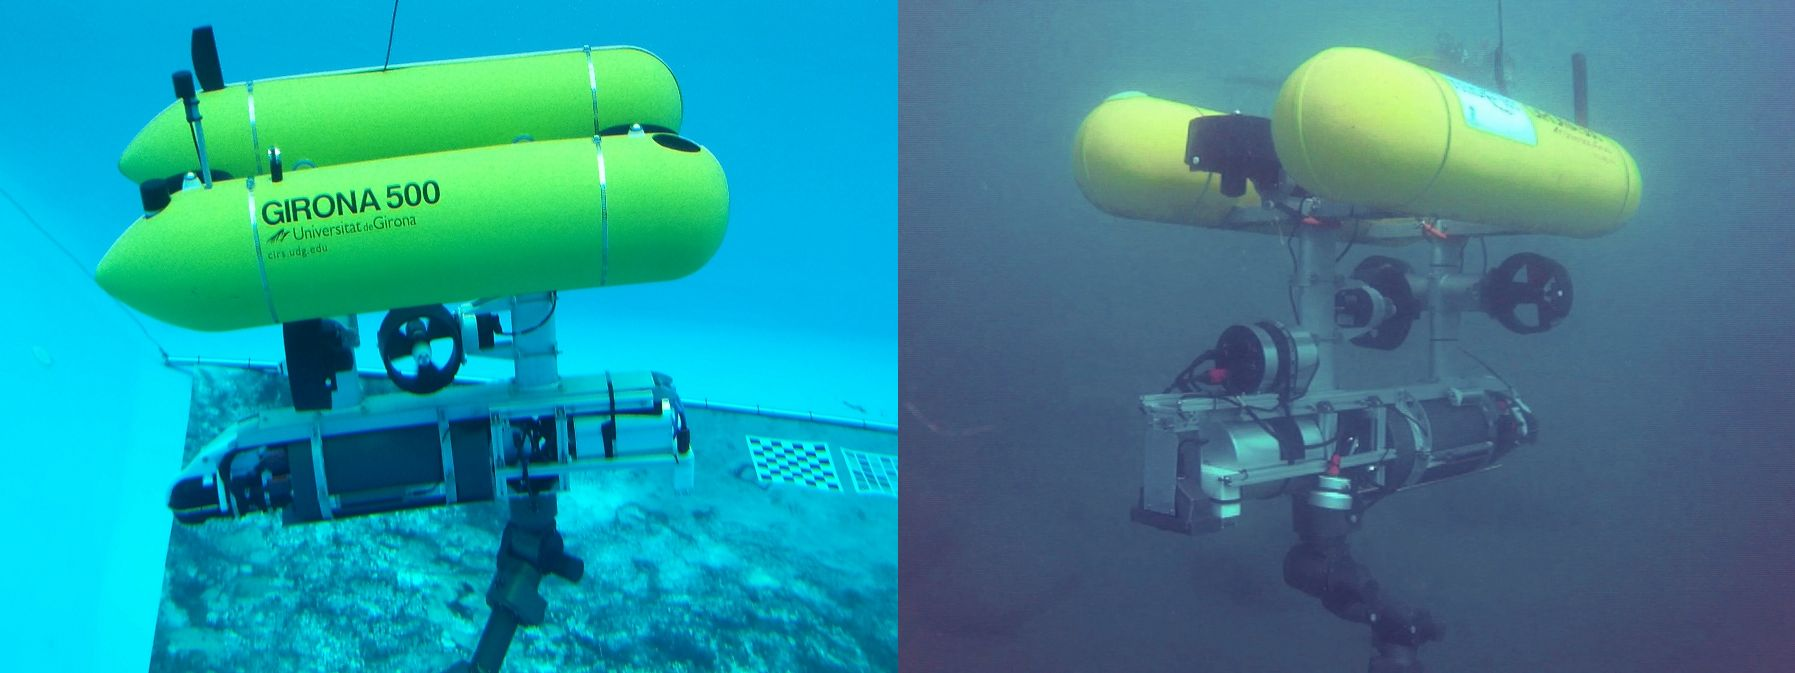
\includegraphics[width=1.000\linewidth]{images/G500-Experiments.jpg}}
  \caption{The Girona 500 AUV during laboratory and harbour experiments. The white box in the front of the lower part is the stereo camera. The cylinder right next to it contains the image processing unit.}
  \label{g500}
\end{figure}

The experiments carried out use data gathered during the TRIDENT project\footnote{See \url{http://www.irs.uji.es/trident/}} both in laboratory and harbour conditions using the Girona500 AUV \cite{Ribas2012} as vehicle (Figure \ref{g500}). Figure \ref{sample-images} shows some example images from both sequences. Ground truth for the laboratory experiment is extracted by matching each image that has been captured against the known image that is printed on the floor of the test pool. As the size of the print is known, 6 DOF camera poses can be computed minimizing reprojection errors of matched features.
\begin{figure}
  \noindent\makebox[\linewidth][c]{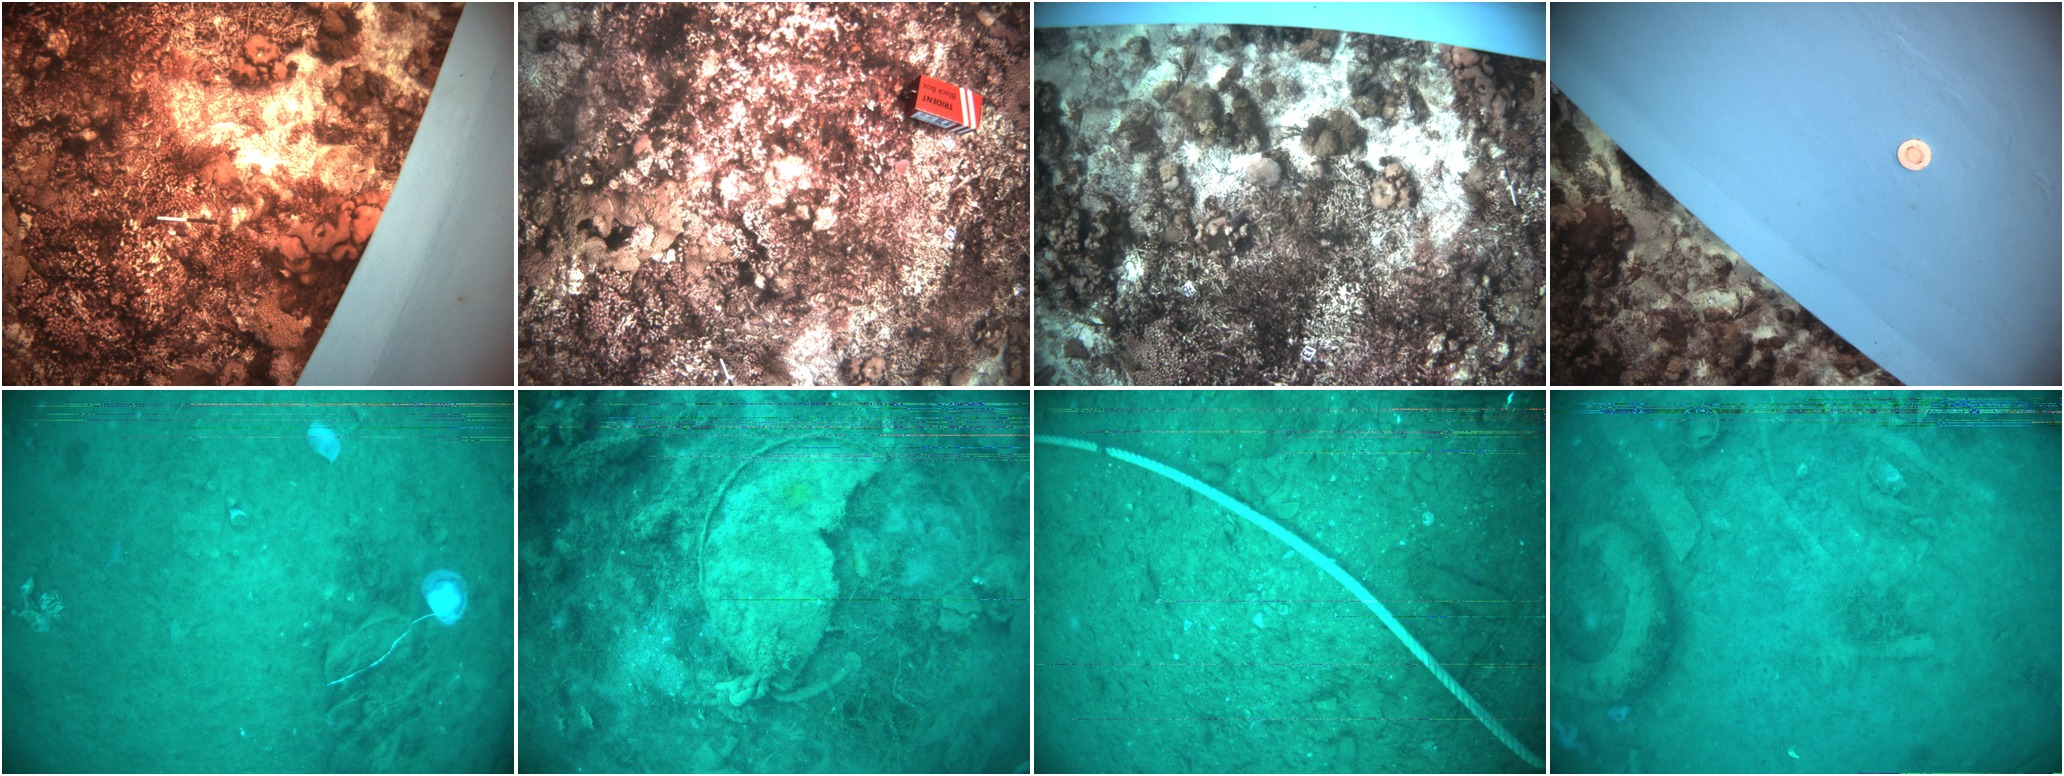
\includegraphics[width=1.000\linewidth]{images/sample_images.jpg}}
  \caption{Sample images from the sequences during the laboratory (top row) and harbour (bottom row) experiments.}
  \label{sample-images}
\end{figure}

For the harbour experiment, the determination of ground truth is more difficult, as no external sensors have been used and positions of natural landmarks are not known. One aim of the project was the construction of a consistent seabed mosaic (see \cite{Ferrer2007}). The computation of this mosaic includes global optimization of all camera poses. The resulting trajectory does not suffer from drift and is therefore chosen as our ground truth reference.

In the harbour experiment, a DVL and an AHS have been used as navigation sensors to let the vehicle follow a previously defined trajectory autonomously. In the laboratory experiments, the vehicle has been remotely controlled by a human operator. Table \ref{experiment-details} summarizes the characteristics of the experiments.

The AUV was configured to not control pitch, roll and sway. Motions in these degrees of freedom are therefore rather small and we cannot compute reasonable error measures for them.

TODO Update plots to contain output from both odometry algorithms with (manually) optimized parameters. Add the plot of the trajectory?

A comparison of linear velocity estimates to ground truth can be found in Figure \ref{error-plots-viso2}. Note that the estimated angular velocities hardly differ from the ground truth throughout the whole path ... for both odometers?

\begin{table}[ht]
  \caption{Experiment details}
  \label{experiment-details}
  \begin{tabular}{l*{3}{c}r}
    & \textbf{CIRS Lab} & \textbf{Roses Harbour}  \\
    \hline
    Total Trajectory Length (m)     & 47.54 & 90.48  \\[3pt]
    Average Velocity (m/s)          & 0.15 & 0.12  \\[3pt]
    Average Altitude (m)            & 1.59 & 1.34  \\[3pt]
    Average Depth (m)               & 2.98 & 1.46  \\[3pt]
  \end{tabular}
\end{table}

TODO Brief description of parameter tuning

TODO Error comparison (table)

TODO Runtime comparison (table)

TODO describe difficulties / explain obvious errors in the data etc.


\section{Conclusion
  \label{conclusion}
}

Visual odometry is a method for motion estimation that gives good results using a low-cost sensor in reasonable conditions. We presented open source wrappers for two publicly available visual odometry algorithms to the community that ease the integration into existing robotic platforms.
We have shown that these algorithms can be used in an underwater environment if both the visibility conditions and the appearance of the sea floor result in images with sufficient texture. Like all incremental motion estimation methods, visual odometry suffers from drift and has to be combined with other sensors to get precise long-term position estimates. Apart from that, failure might occur in situations with insufficient texture, motion blur, or bad visibility.

Despite the mentioned drawbacks we have shown that a visual odometer using a downward looking stereo camera can be a valuable sensor for underwater vehicles giving good estimates for linear movement and rotation about the vehicle's vertical axis.

TODO Complete with experiment results.

% references section
\bibliographystyle{IEEEtran}
\bibliography{references}

% that's all folks
\end{document}


